% Chapter 4

\chapter{Inverse Finite Element Method for Material Parameter Identification} % Main chapter title
\label{iFEMthesis} % For referencing the chapter elsewhere, use \ref{Chapter1} 

The verification of the computational model in the previous chapter was followed by the implementation
of the Inverse Finite Element Method (iFEM) for material parameter identification.
As outlined in Chapter \ref{chapter:computationalmodel}, the Neo-Hookean material model
was employed due to its ability to describe the behavior of ultra-soft polyurethane over 
the range of the considered deformations. Moreover, in Subsection \ref{subsection:inverseFEMtheory} 
the iFEM importance for identifying material parameters for soft materials was explained.\\

In this chapter, the process of parameter identification 
using this technique will be detailed. Firstly, the initial parameter estimation process will be discussed, 
followed by the optimization process. This revolved around iteratively refining the material parameters
to achieve the best match to the experimental load-displacement data of EM II. The two methods 
explored were ANSYS Response Surface Optimization (RSO) and a custom MATLAB routine. Lastly, the implementation 
and development of these optimization strategies, and their strengths and weaknesses, 
will be discussed. 

%----------------------------------------------------------------------------------
\section{Response Surface Optimization}
The Response Surface Optimization is a technique used in ANSYS for optimizing a design by creating 
a response surface, which represents the relationship between the design variables and the objective 
function or performance criteria. The objective of this feature is to find the optimal set of design 
variables that maximize or minimize the objective function.

The process to find parameters using the RSO in ANSYS generally involves the following steps:
\begin{enumerate}
    \item Define the design variables: The variables that influence the design are identified, e.g., geometric parameters, material properties.
    \item Define objective function: The parameter or objective which will be maximized or minimized is defined, e.g., stress, force reaction, volume. 
    \item Define constraints: Constraints or limitations are specified, such as lower or upper bounds.
    \item Generate Design of Experiments (DOE): Set of sample points are generated by varying the design variables. The DOE aims to set a design a space efficiently to capture the relationships between the input and output parameters. Simulations are then performed for each set of design variables in the DOE.  
    \item Create a Response Surface: Based on the results of the simulations, the software constructs a surface by interpolating the discrete sampling points from DOE.
    \item Optimize the design: The optimal set of design variables are searched with optimization algorithms by iteratively evaluating the response surface and adjusting the design variables. The default optimization algorithm in ANSYS is the Multi-Objective Genetic Algorithm (MOGA), which supports multiple objectives and constraints. This algorithm aims to find a global optimum for the given problem \cite{Grebenisan2017}.
    \item Verify the candidate points: The given candidate points from the optimization tool are verified to observe if these satisfy the constraints and meet the target criteria.
\end{enumerate}

For this research, the design, or input variables were the material properties from the Neo-Hookean 
material model, the shear modulus $\mu$ and the incompressibility parameter $D_1$. The output parameters 
were the maximum force reaction in Z-direction $F_z$ and the maximum directional deformation in Z-direction $u_z$.

Based on the observation made in Chapter \ref{chapter:experimentalmodel} regarding the impact of the force 
components in EM II, only the values for the Z-direction were considered. Consequently, the other force 
components could be neglected for this particular case. The prioritization of the Z-direction values came from 
their maximal influence on the outcomes.

\subsection*{Initial Parameter Range}
The initial parameter ranges for the input variables of the RSO were established based on literature review.
Ultra-soft polyurethane, depending on its composition, can have a wide range of mechanical properties \cite{Wendels2021}.
From the literature review a Young's modulus range for this material was \SIrange{10000}{100000}{\pascal}, and the 
Poisson's ratio range was \SIrange{0.36}{0.49}{}. As derivated in the previous chapter in 
Subsection \ref{subsection:level2cmI} with the equations \ref{eq:mucp1}, \ref{eq:bulkmodcp1}, 
and \ref{eq:incomparcp1}, the shear modulus $\mu$ and the incompressibility parameter $D_1$ ranges were calculated.
The corresponding full ranges (FR) were \SIrange{3356}{36765}{\pascal} and \SIrange{1}{168}{\mega\pascal\tothe{-1}}, respectively.

\subsection*{Sensitivity Analysis}
The RSO generated a response surface that enabled the performance of a sensitivity analysis.
The sensitivity analysis helped identify which design variables had the most impact 
on the objective function or performance metric, i.e., it was possible to observe how much 
an objective changed when each input variable changed. By evaluating the sensitivity of the 
function to variations in the design variables, it was possible to prioritize the most 
influential parameters and understand their influence in the model during the optimization 
process.

By examining a local sensitivity bar diagram and a response surface, the sensitivity analysis was conducted.
Figure \ref{fig:fullrangelocalsensi} displays the local sensitivity bar diagram for the design variables
$\mu$ and $D_1$, in relation to the output parameters, namely the maximum force reaction in Z-direction $F_z$ 
and the maximum directional deformation in Z-direction $u_z$. 

The local sensitivity bar diagram provided a quantitative measure of the relative impact of the material 
parameters. This diagram indicated that the shear modulus has a positive correlation with both the force
reaction and the directional deformation. I also highlighted the considerably greater impact of the shear modulus 
on the force reaction, nearly four times as much as the incompressibility parameter. Moreover, $D_1$ exhibited 
an inverse negative correlation with force reaction.
In terms of deformation, both $\mu$ and $D_1$ showed a positive correlation. However, the impact of the 
shear modulus slightly surpassed that of the incompressibility parameter.\\

\begin{figure}%
    \centering
	\begin{tikzpicture}
	\begin{axis}[
	    ybar,
	    bar width=1cm,
	    ymax=80,
	    xlabel=Parameter,
	    ylabel={Local Sensitiviy (\%)},
	    xtick=data,
	    xticklabels from table={Table/sensitivity/fullrangeplat2points/test.csv}{Name},
	    enlarge x limits=1,
	    width=0.8\textwidth,
	    height=6cm,
	    legend style={at={(0.5,-0.15)},
	    anchor=north,legend columns=-1},
	    ymajorgrids=true,
	    grid style=dashed,
	]
	\addplot table [x expr=\coordindex, y=P3] {Table/sensitivity/fullrangeplat2points/test.csv};
	\addplot table [x expr=\coordindex, y=P5] {Table/sensitivity/fullrangeplat2points/test.csv};
	\legend{Directional Deformation, Force Reaction Z Axis}
	\end{axis}
	\end{tikzpicture}
	\caption[Local sensitivity analysis - Initial parameter range]{Local sensitivity analysis displaying the influence of the shear modulus and incompressibility parameter for the directional deformation and force reaction in Z-direction.}%
	\label{fig:fullrangelocalsensi}%
 \end{figure}

The response surface (Fig. \ref{fig:rsoforce}) 
reinforced the findings obtained from the local sensitivity diagram. The steeper gradient of the shear modulus 
signified its greater impact on the force reaction. The incompressibility parameter, on the other hand, 
exhibited a steeper slope at the beginning, but it tended to flatten and almost converged. This indicated 
a lowering influence on the force reaction.

\begin{figure}%
	\centering
   \quad
   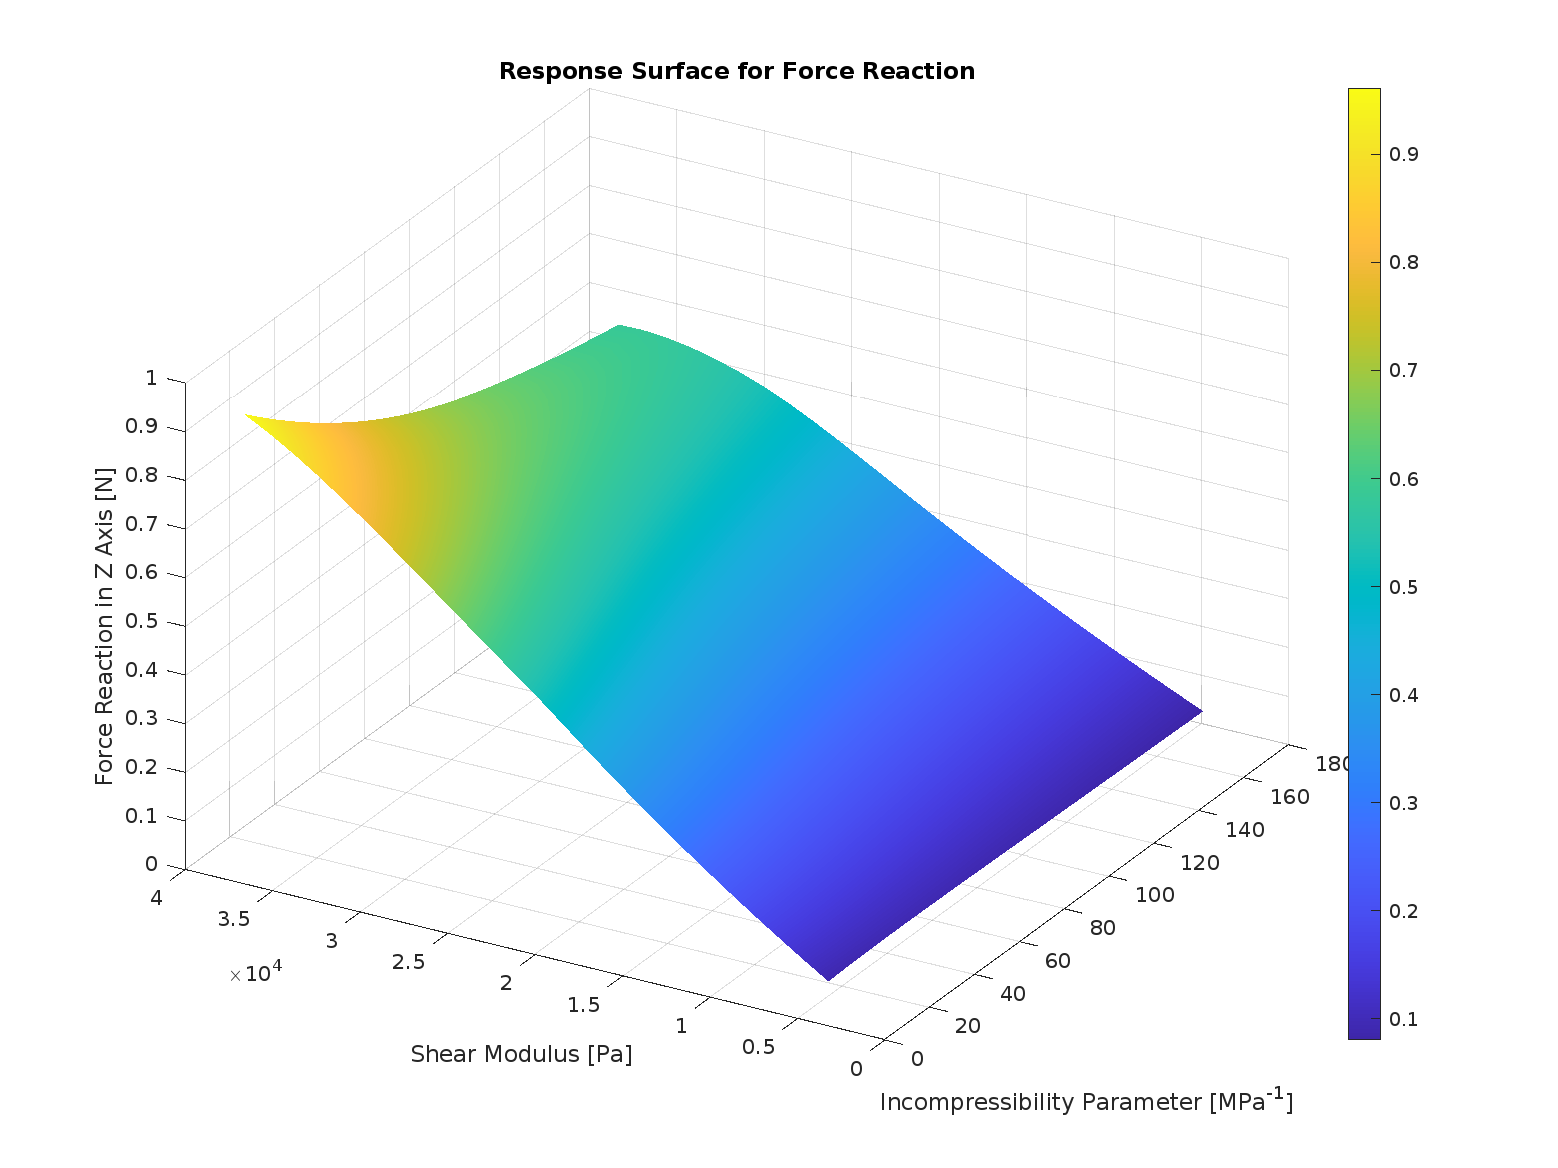
\includegraphics[width=10cm]{Images/ifem/plat NH 4 and 2 fullrange/rsoforce1.png}%
   \caption[Response surface - Force Reaction]{Response Surface for the Neo-Hookean parameters $\mu$ and $D_1$ in relation to the force reaction in the Z-axis.}%
   \label{fig:rsoforce}%
\end{figure}

\subsection*{Initial RSO Results and Analysis}
The primary performance metric or objective for the RSO was to match the maximum force in the Z-direction, 
observed experimentally at a displacement of $u_z=\SI{4}{\milli\meter}$.
The initial RSO process offered three candidate sets of material parameters, with shear modulus values 
around \SI{0.011}{\mega \pascal} and incompressibility parameter values of \SI{50}{\mega\pascal\tothe{-1}}, 
\SI{112}{\mega\pascal\tothe{-1}}, and \SI{161}{\mega\pascal\tothe{-1}}. Nevertheless, these candidates 
did not match with the experimental maximum force when verified. Moreover, it was observed that ANSYS 
tended to offer only higher values for $D_1$ and ignored the lower half of the range. This led to a decision to 
refine the parameter ranges further.\\

The refined or reduced ranges (RR) were from \SIrange{7500}{9500}{\pascal} for the shear modulus and 
\SIrange{1}{10}{\mega\pascal\tothe{-1}} for the incompressibility parameter. The new candidates from the RSO had a 
$\mu$ around \SI{0.085}{\mega \pascal} and $D_1$ of \SI{2}{\mega\pascal\tothe{-1}}, 
\SI{5}{\mega\pascal\tothe{-1}}, and \SI{7}{\mega\pascal\tothe{-1}}. 

Furthermore, it was observed that the maximum total deformation of the specimen did not fully reach the  
displacement of \SI{4}{\milli\meter}, therefore a new target was modified and set for a displacement 
of $u_z\approx\SI{3.9}{\milli\meter}$.

\subsection*{Assessment and Process Optimization}
For each simulation curve obtained, the Root Mean Square Error (RMSE) was calculated.
The RMSE is considered a commonly used metric to evaluate the differences between the predicted and 
observed values in the experiments. This function measured the standard deviation of the residuals 
or prediction errors. The RMSE is given by the formula 
\begin{align}
	\text{RMSE} = \sqrt{\frac{1}{n}\sum_{i=1}^{n}(y_i - \hat{y}_i)^2}\, ,
    \label{eq:rmse}
\end{align}
where $y_i$ is the observed or experimental value, $\hat{y}_i$ is the predicted or simulated value, and 
$n$ is the number of data points. However, since the RMSE is scale-dependent, it was normalized by dividing the
RMSE value with the mean of the observed values%difference of the maximal and minimal value of the observed data
%\begin{align}
%	\text{NRMSE} = \frac{\text{RMSE}}{y_{max} - y_{min}} \, .
%\end{align}
\begin{align}
	\text{NRMSE} = \frac{\text{RMSE}}{\bar{y}} \, .
    \label{eq:nrmse}
\end{align}
Although the RSO proved to be useful, the obtained candidates were not providing a satisfactory 
match to the entire load-displacement curve when using only a single point as the optimization target.
This motivated the introduction of more targets along the curve in addition to the force reaction at 
$u_z=\SI{3.9}{\milli\meter}$, specifically at $u_z=\SI{2}{\milli\meter}$, 
and later an additional target at $\SI{3}{\milli\meter}$ was also tested.\\

Initially, the force reactions at \SI{2}{\milli\meter} and \SI{4}{\milli\meter} indentation depths
were used as targets. The range of the shear modulus for this two-point (2P) target was set to
\SIrange{6000}{10000}{\pascal}, while the range of the incompressibility parameter was set to 
\SIrange{1}{6}{\mega\pascal\tothe{-1}}.

Subsequently, a third target was introduced at \SI{3}{\milli\meter} indentation depth, and the ranges 
for $mu$ and $D_1$ were revised to \SIrange{9000}{15000}{\pascal} and \SIrange{1}{50}{\mega\pascal\tothe{-1}}, 
respectively.

The RSO for the two-point target optimization gave a $\mu_{2p}=\SI{9999.7}{\pascal}$ and a 
$D_{1_{2p}}=\SI{5.8}{\mega\pascal\tothe{-1}}$. In comparison, the three-point (3P) target optimization 
yielded a  $\mu_{3p}=\SI{10867}{\pascal}$ and $D_{1_{3p}}=\SI{47.2}{\mega\pascal\tothe{-1}}$.

Despite the differences in the estimated material parameters, the simulation curves obtained  
from these parameter sets were nearly identical, as shown in Figure \ref{fig:1vs2vs3points}.
Furthermore, the RSO exhibited the tendency to select higher values from the range of the 
incompressibility parameter.

%Figure% shows the comparison between matching the data ith one point vs 2 and 3 points 
%showed the result of introducing an extra optimization target in the RSO. 
%The use of \SI{2}{} or even \SI{3}{} target points along the curve did not showed a significant
%difference in the give material paremeter set for load-displacement curve.
\begin{figure}%
    \centering
   \quad
    \begin{tikzpicture}[scale=1]
        \begin{axis}[
            xmax=4.2,xmin=0,
            ymin= 0,ymax=0.6,
            ytick={0,0.1,0.2,...,0.5},
            xlabel={Displacement $u [mm]$},
            ylabel={Force reaction $F_{II} [N]$},
            grid = major,
            legend pos= north west]
            \addplot+[smooth, no markers, thick] table [y=$Force$, x=Def]{Table/RSO/expdatatop.dat};
            \addplot+[smooth, no markers, thick] table [y=$Force$, x=Def]{Table/RSO/2point99997_6.dat};
			\addplot+[smooth, no markers, thick] table [y=$Force$, x=Def]{Table/RSO/3point10867_47.dat};
            \legend{Experiment II,RSO-2 points,RSO-3 points}
        \end{axis}
    \end{tikzpicture}%
   \caption[Multi-objective optimization comparison]{Analysis of multi-objective target optimization, \SI{2}{} and \SI{3}{} sought targets were introduced in the RSO process. }%
   \label{fig:1vs2vs3points}%
\end{figure}

Given that the two-point and three-point target optimizations had comparable results, the optimization
was continued with the two-point target optimization. This decision was driven when considering 
the computational cost, as this requires fewer simulations than the three-point target optimization.

%buscar un ejemplo con un grafico mostrando dos puntos y un punto
%explicar cambio en sets

\section{Minimizing the Objective Function}

In addition to the RSO, a separate identification process was conducted with MATLAB to find the global minimum of 
the objective function. The objective function was defined as the NRMSE, which quantifies the difference 
between the simulated and experimental responses.

The MATLAB optimization used the data from the RSO calculated error measurements to approximate 
the objective function as a surface in a three-dimensional space in relation to the design variables. 

Using data from approximately \SI{35}{} simulations, a surface was generated where the X-axis represented the shear 
modulus, the Y-axis represented the incompressibility parameter, and the Z-axis represented the NRMSE 
of each simulation. The Mean Relative Error (MRE) 
\begin{align}
	\text{MRE} = \frac{1}{n} \sum_{i=1}^{n} \left| \frac{y_i - \hat{y}_i}{y_i} \right| \, ,
    \label{eq:mre}
\end{align}
was also calculated for each simulation, and the same surface approximation method was applied. 
The approximation was performed with a second and fourth degree polynomial.
Figure \ref{fig:poly4NRMSE}
shows the surface plot of a fourth-degree polynomial with \SI{15}{} variables for the NRMSE. 
The fourth degree polynomial function had the following form
\begin{align}
	\begin{split}
	f(x) = p00 + &p10x_1 + p01x_2 + p20x_1^2 + p11x_1x_2 + p02x_2^2 + \\
	&p30x_1^3 + p21x_1^2x_2 + p12x_1x_2^2 + p03x_2^3 + \\
	&p40x_1^4 + p31x_1^3x_2 + p22x_1^2x_2^2 + p13x_1x_2^3 + p04x_2^4 \,.
	\end{split}
\end{align}
%Evtl surface beeschreiben poly2 doesnt reach tiefsten punkten...
\begin{figure}
    \centering
    \begin{subfigure}[b]{0.45\textwidth}
    \centering
    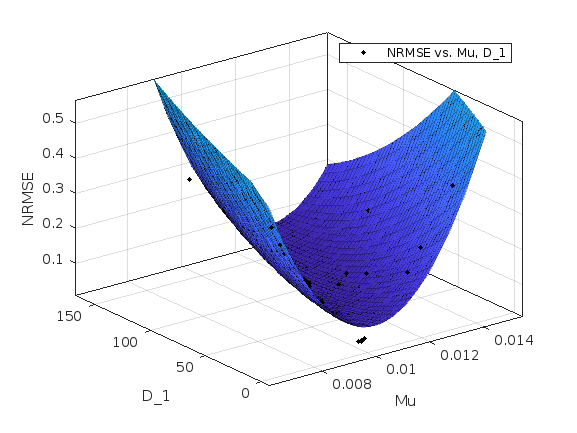
\includegraphics[width=\textwidth]{Images/ifem/MATLAB/NRMSE2poly.png}
    \caption{Second degree polynomial surface}
    \label{fig:poly2NRMSE}
    \end{subfigure}
    \hfill
    \begin{subfigure}[b]{0.45\textwidth}
    \centering
    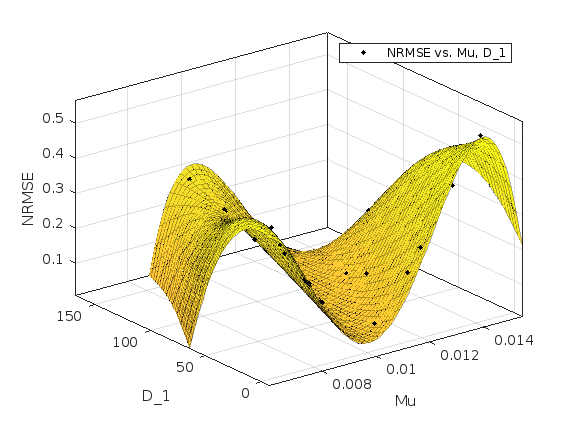
\includegraphics[width=\textwidth]{Images/ifem/MATLAB/NRMSE4poly.png}
    \caption{Fourth degree polynomial surface}
    \label{fig:poly4NRMSE}
    \end{subfigure}
    \hspace{0.3cm}
    \caption[Polynomial approximation surfaces-NRMSE]{Surface approximation method with a second and fourth degree polynomial for NRMSE.}
    \label{fig:poly2and4}
\end{figure}
\begin{figure}
    \centering
    \begin{subfigure}[b]{0.45\textwidth}
    \centering
    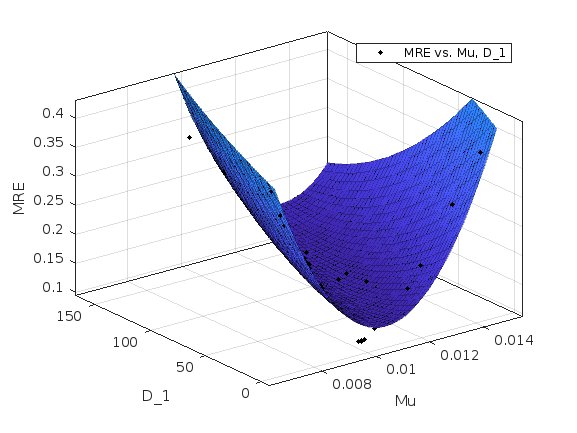
\includegraphics[width=\textwidth]{Images/ifem/MATLAB/MRE2poly.png}
    \caption{Second degree polynomial surface}
    \label{fig:poly2MRE}
    \end{subfigure}
    \hfill
    \begin{subfigure}[b]{0.45\textwidth}
    \centering
    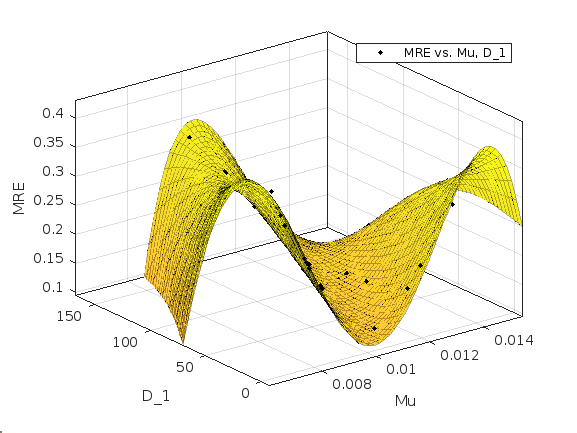
\includegraphics[width=\textwidth]{Images/ifem/MATLAB/MRE4poly.png}
    \caption{Fourth degree polynomial surface}
    \label{fig:poly4MRE}
    \end{subfigure}
    \hspace{0.3cm}
    \caption[Polynomial approximation surfaces-MRE]{Surface approximation method with a second and fourth degree polynomial for MRE.}
    \label{fig:poly2and4MRE}
\end{figure}
The results obtained from the different polynomial degrees and the two performance metrics were summarized
in Table \ref{tab:materialsetMATLAB}.
\begin{table}[h!]
	\centering
	\begin{tabular}{|c|c|c|c|}
	\hline
	\textbf{Polynomial Degree} & \textbf{Error Metric} & $\mu$ (Pa) &	$D_1$ (MPa\textsuperscript{-1}) \\
	\hline
	2 & NRMSE & 12200 & 108.6 \\
	4 & NRMSE & 10600 & 29.6 \\
	2 & MRE & 11900 & 72.7 \\
	4 & MRE & 10200 & 1.1 \\
	\hline
	\end{tabular}
	\caption[Material parameter sets obtained from MATLAB]{Shear modulus and incompressibility parameter obtained from different polynomial degrees and error metrics using MATLAB script.}
	\label{tab:materialsetMATLAB}
\end{table}

This revealed that varying the polynomial degree and the performance metric can influence the estimated material parameters. 
A higher polynomial degree tended to result in a lower shear modulus and incompressibility parameter. Furthermore, 
using the MRE as the performance metric resulted in lower estimates for these parameters.\\

\section{Comparison between RSO and MATLAB Optimization}
\label{section:comparisonrsomatlab}

During the parameter identification exploration process, both RSO and MATLAB-based optimization proved to be valuable tools with 
their own distinct strengths and weaknesses. The combined use of these methods complemented the overall analysis of their application in the
iFEM process.\\

The RSO in ANSYS provided a relatively user-friendly interface which did not require a background in programming, while its integration
in ANSYS generated an intuitive workflow. Moreover, the RSO included built-in tools for the sensitivity analysis, which provided 
valuable information and insights into the relationship between the design variables and the output parameters. 
However, the RSO offered less flexibility compared to a custom-coded MATLAB optimization routine, and there was the need to 
reduce the number of the design variables and their constraints to achieve an adequate result.\\

MATLAB strengths relied on its highly customizable approach for problem-sol-\\ving. 
In addition, the advanced tools for data 
analysis and visualization were useful to generate some direct relationship with the performance metrics. Still, 
MATLAB demanded software expertise, and importing the data from ANSYS introduced some time cost. Furthermore, for an 
accurate polynomial approximation, an increase in data points and preparation was necessary.\\

In conclusion, the choice between RSO and MATLAB optimization depends on the specific requirements of the study, 
the complexity of the problem, and the resources and skills available. 
This study complemented both methods to provide a more comprehensive parameter estimation.
Consequently, the best material parameters identified through the RSO and the MATLAB-based optimization were 
inserted into the computational model for evaluation. The performance of these parameter sets was compared against 
the experimental data to determine their suitability.

%\section{Material Modeling}
%In an ideal and first scenario, this material can be assumed as linear, isotropic, 
%elastic and nearly imcompressible. For this case, there are two main variables, the Young's
%Modulus \(E\), and the Poisson's ratio $\nu$.
%
%%comentario sobre la influencia del bulk modulus y poissons ratio
%From the parametric analysis, it is possible to see that the bulk 
%modulus of this material does not possess a big impact in the FE 
%simulation results. This conclusion combined with the results 
%from the Poisson ratio in the first material model coincide with the 
%statements from Bergström, where it is no vital to know these parameters 
%to obtain accurate FE computational models, as these have limited
%influence on the mechanical response. \cite{Bergström2015} %pag64Bergströom




%----------------------------------------------------------------------------------
%\subsection{Objective Function Optimzation}

%\subsection{Analysis and Comparison of Each Approach}

%---------------------------------------------------------------------------------
